\section{Dynamic Community Discovery}
    
    Abbiamo analizzato vari algoritmi di Community Discovery, selezionandone uno al fine di condurre al meglio il nostro studio. Mostriamo quindi il susseguirsi di eventi che rappresentano l'evoluzione delle comunità nel tempo in tutta la rete. 
    
    
     \begin{table*}[b]
        \small
        \centering
        \caption{Funzioni di \textit{scoring} utilizzate: N: \textit{Total Nodes in Community}; E: \textit{Total Edges in Community}; AID: \textit{Average Internal Degree}; ID: \textit{Internal Density}; GNM: \textit{Girvan-Newman Modularity}; C: \textit{Conductance}; NC: \textit{Normalized Cut}; TPR: \textit{Triangle Participation Ratio}. In basso: \textit{Coms\_T1}: numero di comunità iniziali al tempo 1;\textit{ Max\_coms}: numero massimo di comunità raggiunto nei vari \textit{snapshot}; \textit{Final\_coms}: numero di comunità finali.}
        \label{table:Community}
        \rowcolors{1}{}{lightgray}
        \resizebox{\textwidth}{!}{%
        \begin{tabular}{|c|cccccc|} 
        \hline
                    & Louvain & Label Propagation & Angel   & Demon    & WalkTrap & Infomap  \\ 
        \hline
        N           & 63.40   & 20.49             & 164.59  & 227.01   & 18.57    & 70.06   \\
        E           & 135.94  & 51.68             & 839.42  & 1513.23  & 38.41    & 204.58   \\
        AID         & 1.60    & 1.70              & 3.12    & 7.08     & 1.60     & 1.37    \\
        ID          & 0.79    & 0.75              & 0.63    & 0.29     & 0.68     & 0.86    \\
        GNM         & 0.63    & 0.56              & -0.20   & 0.13     & 0.54     & 0.45    \\
        C           & 0.04    & 0.27              & 0.33    & 0.65     & 0.31     & 0.01    \\
        NC          & 0.04    & 0.27              & 0.33    & 0.73     & 0.31     & 0.01    \\
        TPR         & 0.17    & 0.25              & 0.87    & 1.00     & 0.21     & 0.14    \\ 
        \hline
        \hline
        Coms\_T1    & 16     & 16                 & 6       & 6        & 16       & 16       \\
        Max\_coms   & 263    & 851                & 48      & 166      & 898      & 238      \\
        Final\_coms & 263    & 814                & 48      & 166      & 898      & 238      \\
        \hline
        \end{tabular}
        }
    \end{table*} 
    
    \subsection{Valutazione e selezione dell'algoritmo di Community Discovery}\label{val}
    
    Il concetto di comunità non trova, ad oggi, una definizione univoca, per cui, prima di scegliere quale algoritmo utilizzare nella ricerca delle comunità della rete, abbiamo voluto approfondire e analizzare alcuni degli algoritmi implementati nella libreria Python {\scshape CDlib}, e in particolare: \textit{Louvain}, \textit{Label-propagation}, \textit{Angel}, \textit{Demon}, \textit{Walk Trap} e 
    \textit{Infomap}.  
    I confronti tra questi sono stati effettuati attraverso alcune \textit{fitness function}, tra cui il punteggio NF1 (fig. \ref{heatmap_algoritms}) e diverse funzioni di \textit{scoring} (tab. \ref{table:Community}), utilizzate per valutare la bontà delle divisioni in comunità ottenute.
    La figura \ref{heatmap_algoritms} evidenzia un'alta corrispondenza fra gli algoritmi \textit{Louvain} e \textit{Infomap} e fra \textit{Label-propagation} e \textit{Walk Trap}.
    
    \begin{figure}
        \centering
        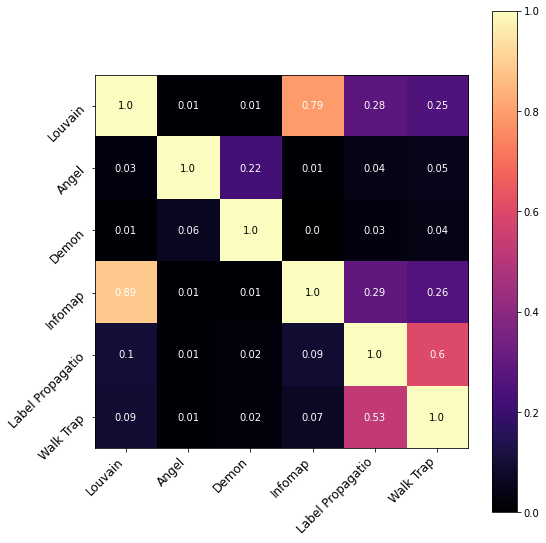
\includegraphics[width=7cm] {4_Community_discovery/heatmap.png}
        \caption{Risultati delle correlazioni tra gli algoritmi secondo il punteggio NF1.}
        \label{heatmap_algoritms}
    \end{figure}
    
   Quasi tutti gli algoritmi effettuano una prima suddivisione identica, inizializzando sedici comunità, ad eccezione degli algoritmi \textit{Angel} e \textit{Demon} che ne individuano sei.
   
   Sulla base dei risultati ottenuti, abbiamo scelto di concentrare la nostra analisi su tre algoritmi: \textit{Louvain}, \textit{Angel} e \textit{Demon}. 
   Il primo denota un buon punteggio dell'indice di Girvan-Newman, che conferisce una miglior previsione tra gli \textit{edge} attesi in relazione a quelli effettivamente valutati durante la stima delle comunità. 
   Tuttavia, produce un punteggio di \textit{Triangle Participation Ratio} molto basso rispetto a tutti gli altri algoritmi, evidenziando una scarsa presenza di triplette nelle comunità.
   Per quanto riguarda gli algoritmi \textit{Angel} e \textit{Demon}, la loro rilevanza sta nel fatto che collezionano i punteggi più elevati di \textit{Average Internal Degree}, producendo rispettivamente 46 e 157 comunità finali. D'altro canto, però, Angel è anche l’unico algoritmo che ottiene un punteggio negativo riguardo la \textit{Girvan-Newman modularity}: in ogni comunità, infatti, il numero di \textit{edge} attesi è superiore rispetto a quello effettivo. Da notare è anche l'alta presenza di triplette nelle comunità individuate dai due algoritmi (\textit{Triangle Participation Ratio}). 
   
   \subsubsection{Confronto nel tempo}\label{dcd}
   Abbiamo infine analizzato il modo in cui queste due differenti tipologie di algoritmi selezionino le comunità nel tempo. 
   Per farlo, abbiamo suddiviso il periodo di tempo in cui è avvenuta la raccolta dei dati in sette \textit{frame} temporali, posti a cavallo di ciascuna partita disputata dalla Nazionale Italiana.
   Per tutti gli algoritmi, i risultati ottenuti (fig. \ref{community_evolution}) evidenziano lo \textit{spike} del numero di comunità verificatosi durante le partite Italia-Svizzera e Italia-Galles, ovvero dopo la prima dichiarazione della Nazionale Italiana sul tema dell'inginocchiarsi \cite{inginocchiobonucci}, coincidente all'aumento del numero di nodi della rete (fig. \ref{hubs_evolution}). Il numero di comunità continua a crescere fino alla partita Italia-Austria, dopo la quale si mantiene pressocché costante.
   Alla luce delle analisi condotte, la scelta è ricaduta sull'algoritmo Louvain. In particolare, due sono stati i fattori decisivi: il primo riguarda le analisi in sezione \ref{val}, in principal modo il fatto che il risultato del valore \textit{Girvan-Newman} sia il migliore rende la valutazione delle comunità accettabile; infine usando Louvain abbiamo la possibilità di valutare le comunità sulla base di un valore da noi personalizzato, l’attributo \texttt{weight}, il quale evidenzia quanto sia forte la relazione tra due nodi in base ai contatti che hanno avuto.
    
   \subsection{Come si muovono gli utenti durante il Campionato EURO 2020}
    
    \begin{figure*}
        \centering
        \begin{subfigure}{.45\textwidth}
            \centering
            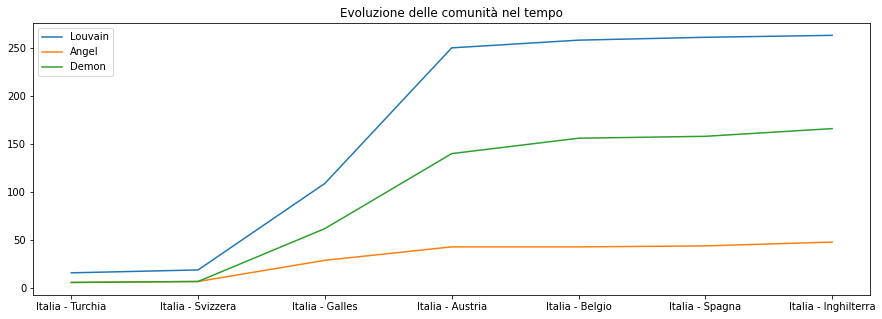
\includegraphics[width=7cm] {4_Community_discovery/community_evolution.png}
        \caption{Numero delle comunità nel tempo.}
        \label{community_evolution}
        \end{subfigure}
        \centering
        %\vspace{-3mm}
        \begin{subfigure}{.45\textwidth}
            \centering
           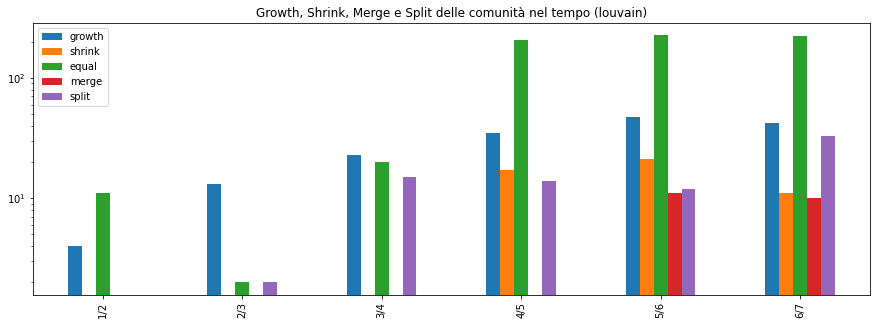
\includegraphics[width=7cm] {4_Community_discovery/log_communities_events.png}
        \caption{Numero e tipo di eventi nel tempo.}
        \label{community_evolution_1}
        \end{subfigure}
        \caption{}
        \label{fig:community}
    \end{figure*}
    
    Utilizzando l’algoritmo \textit{Louvain} sono state definite le comunità ad ogni tempo. Sfruttando l'indice di Jaccard, abbiamo definito una funzione di somiglianza che è stata applicata a tutti i \textit{match} nei nostri vari \textit{frame} temporali, andando così a valutare l'evolversi delle comunità nel tempo. Al fine di analizzare tutti i casi di \textit{merging} e \textit{splitting}, abbiamo applicato la funzione di somiglianza sia dal passato al futuro (da $t$ a $t+1$) che dal futuro al passato (da $t+1$ a $t$).
    
    Una volta valutate le comunità e i vari punteggi di \textit{matching}, abbiamo implementato delle funzioni che potessero eseguire un'analisi in modo semplice e adattare i risultati in un formato che ci fosse congeniale. Per intercettare dai \textit{matches} tutti gli eventi analizzabili (le \textit{growth}, gli \textit{shrink}, i \textit{merge} e gli \textit{Split}), abbiamo creato una funzione chiamata \texttt{community\_evolution(cluster\_community)}, la quale prende come parametro una stringa che identifica il cluster temporale e una comunità all’interno di quel cluster (es. \texttt{community\_evolution(“1\_0”)}). Questa funzione restituisce una prima panoramica testuale di quello che è l’andamento nel tempo della comunità in input, a partire dal dato cluster temporale. L'output infatti sarà un dizionario che ha come chiave "comunità/evento", e come valore un array di una o più tuple che rappresentano l'evento a cui vengono associate una o più comunità corrispondenti (una per tupla) del cluster temporale successivo. La tupla è composta da tre elementi - comunità iniziale, comunità finale nel dato cluster temporale e indice di Jaccard - come nell'esempio seguente:
    
    \begin{lstlisting}[
                    framesep=5pt,
                    xleftmargin = 0pt,
                    xrightmargin = 0pt,
                    framexleftmargin=0pt,
                    framexrightmargin=0pt,
                    frame=tb,
                    framerule=0pt,
                    caption= esempio di output della funzione \texttt{community\_evolution (“cluster\_community”)}, label=output]
    {
       "1_0/simple": [(1_0, 2_0, 1.0)],
       "2_0/split": [(2_0, 3_11, 0.4),(2_0, 3_12, 0.2)],
       "3_11/3_12/merge": [(3_11, 4_0, 0.5), (3_12, 4_0, 0.1)]
       ...
    }
    \end{lstlisting}

    Con la struttura dati definita, abbiamo creato un grafico che raffigurasse le evoluzioni dei vari eventi. 
    Possiamo affermare quindi che, come ci aspettavamo, gli eventi di \textit{growth} e \textit{equal} sono presenti fin da subito nelle comunità e che questi sono anche i due eventi che hanno una maggior frequenza nel tempo. Gli eventi di \textit{split} delle comunità hanno inizio a cavallo tra il tempo $2$ e il tempo $3$. Nell'intervallo $4/5$ si nota come la dimensione di alcune comunità inizi a diminuire. Nell'intervallo $5/6$ le comunità iniziano a unirsi tra loro (fig. \ref{community_evolution_1}).
    
    \begin{figure*}
        \centering
        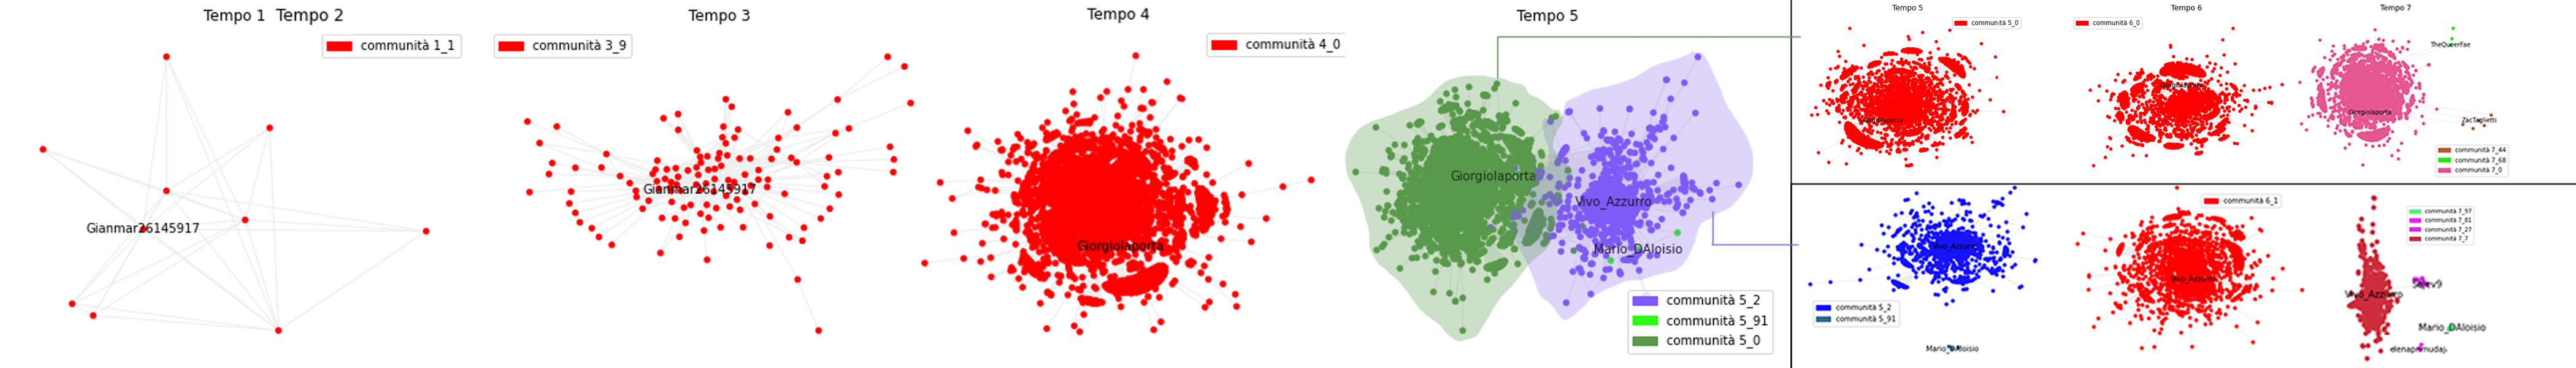
\includegraphics[width=15cm] {4_Community_discovery/evolution.png}
        \caption{Evoluzione di una comunità nel tempo}
        \label{example_community_events}
    \end{figure*}
    
    Servendoci della funzione \texttt{community\_evolution}, abbiamo \textit{plottato} una rappresentazione delle comunità e degli eventi che le caratterizzano nel tempo. Sfruttando l’output della funzione abbiamo estratto i nodi, creando così dei sottografi che evidenziano quello che accade alla comunità in \textit{input} nella transizione tra un tempo e il successivo, fino alla fine dei \textit{frame} temporali. 
    
   In figura \ref{example_community_events}, assistiamo all'evoluzione delle comunità derivanti dalla comunità 1, che, per comodità e leggibilità, etichetteremo con il nome del suo \textit{hub} principale. Fino al tempo 2 la comunità rimane costante, mentre sia al tempo 3 che al tempo 4 assistiamo a dei Growth, e il nodo con la maggiore \textit{degree} cambia da @Gianmar26145917 ($C_{u} = 2.53$) a @Giorgiolaporta ($C_{u} =  1.66$). Al tempo 5 possiamo osservare il primo Split della comunità in tre, con i relativi \textit{hub} principali  @Giorgiolaporta, @Vivo\_Azzurro ($C_{u} = 0$) e @Mario\_DAloisio ($C_{u} = -1$).
   Successivamente troviamo gli eventi di Merge, fra le comunità @Vivo\_Azzurro e @Mario\_DAloisio, e l'evento Shrink della comunità @Giorgiolaporta al tempo 6. Infine rivediamo degli eventi di \textit{split} per entrambi i percorsi.
   
